\section{Modelo Entidad–Relación}

El Modelo Entidad–Relación representa la estructura conceptual de la base de datos desarrollada para el sistema ECOBICI. En este modelo se identifican las principales entidades involucradas en la operación del sistema, así como sus atributos y relaciones.

Las entidades modeladas permiten administrar la información relacionada con usuarios, membresías, bicicletas, estaciones, viajes, incidentes, métodos de pago y personal operativo. Asimismo, se establecen las cardinalidades necesarias para garantizar la correcta representación de las reglas de negocio identificadas durante la fase de análisis.

Como puede observarse en la Figura~\ref{fig:modelo_er}, el modelo conceptual permite identificar claramente las dependencias entre las entidades principales del sistema, sirviendo como base para la construcción del modelo relacional y la implementación física de la base de datos.

\begin{figure}[H]
	\centering
	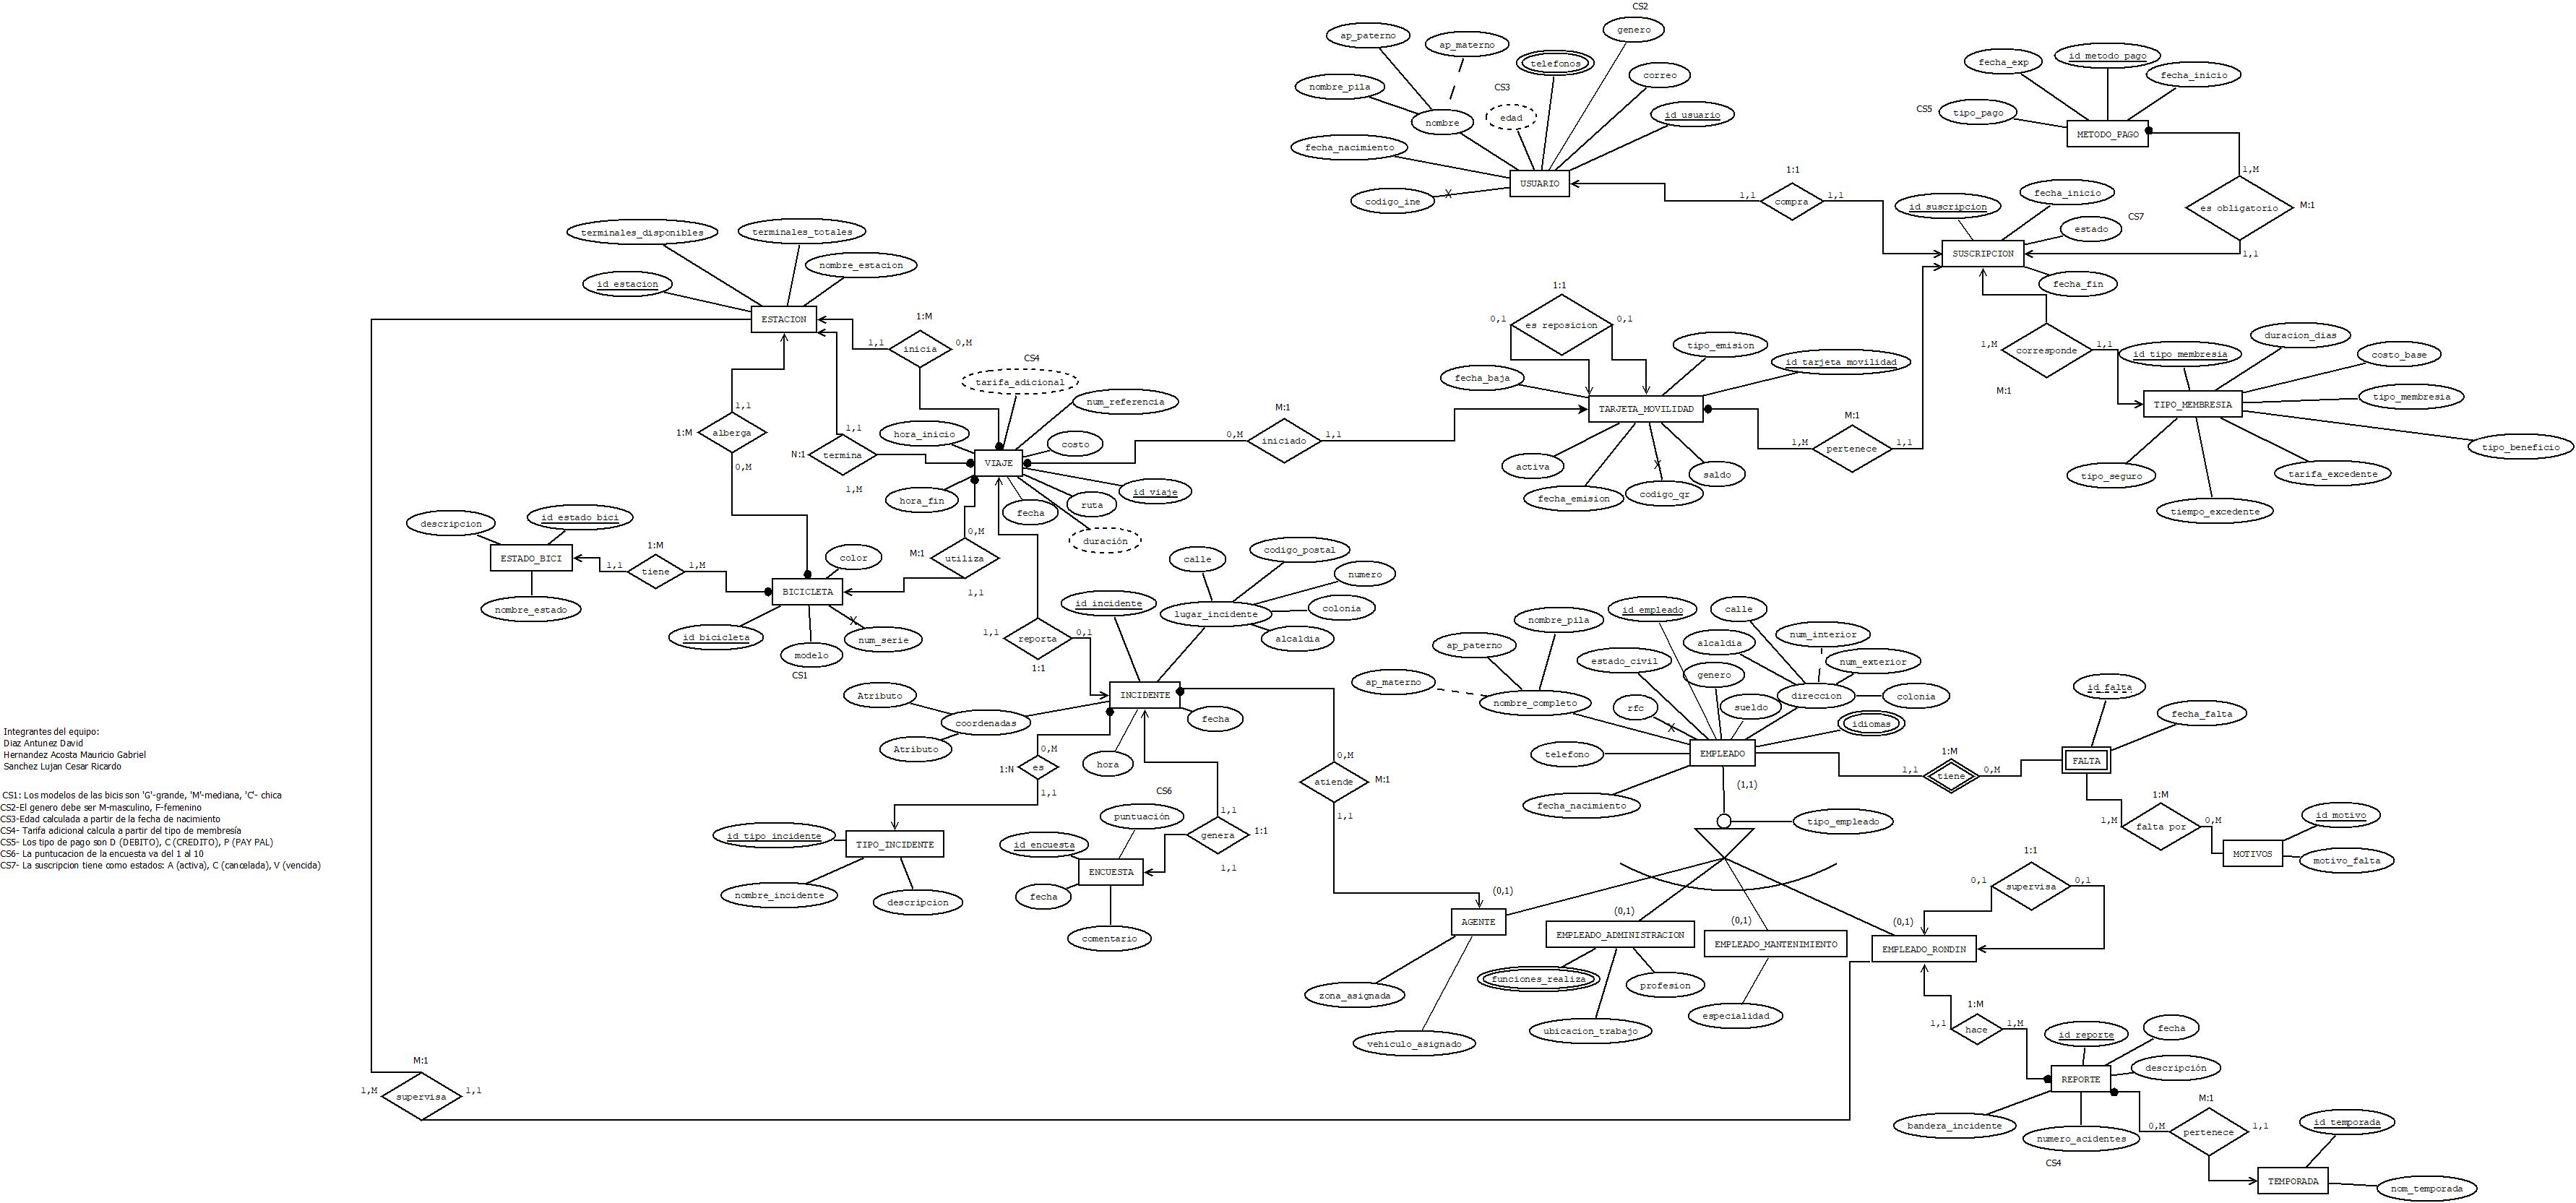
\includegraphics[width=0.9\textwidth]{figures/mer.jpg}
	\caption{Modelo Entidad–Relación del sistema ECOBICI}
	\label{fig:modelo_er}
\end{figure}
